\documentclass[10pt]{beamer}
\usetheme[
%%% option passed to the outer theme
%    progressstyle=fixedCircCnt,   % fixedCircCnt, movingCircCnt (moving is deault)
  ]{Feather}

% If you want to change the colors of the various elements in the theme, edit and uncomment the following lines

% Change the bar colors:
%\setbeamercolor{Feather}{fg=red!20,bg=red}

% Change the color of the structural elements:
%\setbeamercolor{structure}{fg=red}

% Change the frame title text color:
%\setbeamercolor{frametitle}{fg=blue}

% Change the normal text color background:
%\setbeamercolor{normal text}{fg=black,bg=gray!10}

%-------------------------------------------------------
% INCLUDE PACKAGES
%-------------------------------------------------------

\usepackage[utf8]{inputenc}
\usepackage[english]{babel}
\usepackage[T1]{fontenc}
\usepackage{helvet}
\usepackage{array}

%-------------------------------------------------------
% DEFFINING AND REDEFINING COMMANDS
%-------------------------------------------------------
% colored hyperlinks
\newcommand{\chref}[2]{
  \href{#1}{{\usebeamercolor[bg]{Feather}#2}}
}
%-------------------------------------------------------
% INFORMATION IN THE TITLE PAGE
%-------------------------------------------------------

\title[] % [] is optional - is placed on the bottom of the sidebar on every slide
{ % is placed on the title page
      \textbf{Sudo-ku}
}

\subtitle[DM Pro 2016]
{
%      \textbf{v. 1.0.0}
}

\author[Energy]
{      Energieffektivgruppen \\
 %     {\ttfamily dmpro16@samfundet.no}
}

\institute[]
{
%      Faculty of Mathematics, Informatics and Information Technologies\\
%      Plovdiv University ``Paisii Hilendarski''\\

  %there must be an empty line above this line - otherwise some unwanted space is added between the university and the country (I do not know why;( )
}

\date{\today}

%-------------------------------------------------------
% THE BODY OF THE PRESENTATION
%-------------------------------------------------------

\begin{document}

%-------------------------------------------------------
% THE TITLEPAGE
%-------------------------------------------------------

{\1% % this is the name of the PDF file for the background
\begin{frame}[plain,noframenumbering] % the plain option removes the header from the title page, noframenumbering removes the numbering of this frame only
  \titlepage % call the title page information from above
\end{frame}}


\begin{frame}{Content}{}
\tableofcontents
\end{frame}


%-------------------------------------------------------
\section{The Task}
%-------------------------------------------------------

\begin{frame}{The task}
\begin{itemize}
\item Construct a computer that makes use of binarized neural network deployed on an FPGA
\item The BNN should recognize digits
\item Computer must be battery powered
\item Maximize battery life
\item Sudoku solver that displays the board and correctness
\end{itemize}
\end{frame}

%-------------------------------------------------------
\section{Binarized Neural Network}
%-------------------------------------------------------


%-------------------------------------------------------
\section{The Operation of Sudo-ku}
%-------------------------------------------------------

\begin{frame}{The Operation of Sudo-ku}
\centering{
	\includegraphics[height=.7\textheight]{graphics/Lifetime.pdf}
}
\end{frame}


\begin{frame}{The operation of sudo-ku}{Image restraints}
\begin{itemize}
\item White Sudoku board on black background
\item Not rotated more than 45 degrees in any direction
\item Square board
\end{itemize}
\centering{
	\includegraphics[width=50mm,height=.4\textheight]{graphics/foto2.jpg}
}
\end{frame}


%-------------------------------------------------------
\section{Data flow and memory}
%-------------------------------------------------------


\begin{frame}{Data flow and memory}{On the FPGA}
\centering{
	\includegraphics[height=.7\textheight]{graphics/mem_top.pdf}
}
\end{frame}

\begin{frame}{Data flow and memory}{In the Transformer-module}
\centering{
	\includegraphics[height=.7\textheight]{graphics/mem_trans.pdf}
}
\end{frame}


%-------------------------------------------------------
\section{PCB Design}
%-------------------------------------------------------

\begin{frame}{PCB Design}{High Level Schematic}
\centering{
	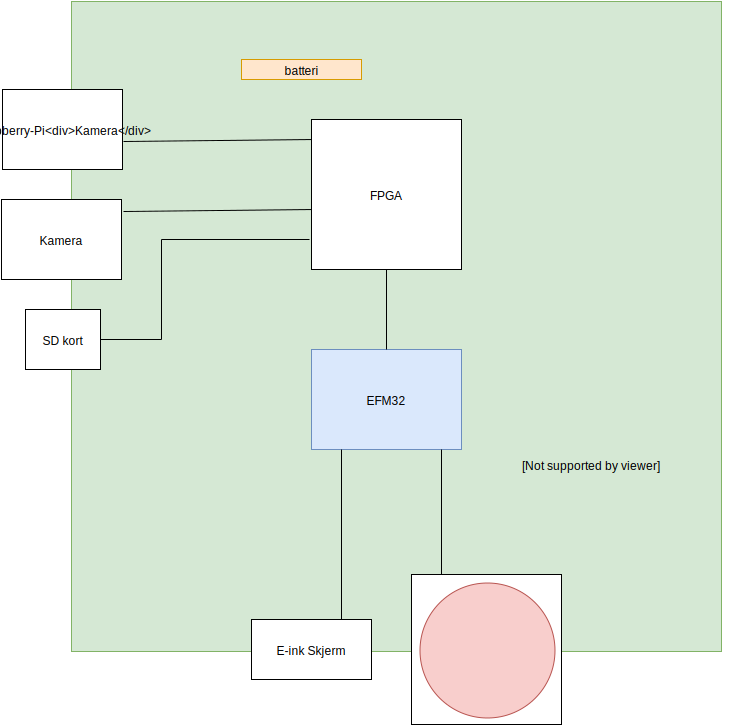
\includegraphics[height=.7\textheight]{graphics/system_overview.pdf}
}
\end{frame}


\begin{frame}{PCB Design}{Energy estimates}
\centering{
\begin{tabular}{ | m{5em} | m{1cm}| m{1cm} | }
\hline
          & Idle      & Load   \\
\hline
Estimated & 0,36W    & 0,48W  \\
\hline
Measured  & 0,77W    & 0,81W \\
\hline
\end{tabular}
}
\end{frame}


\begin{frame}{PCB Design}{3D Drawing}
\centering{
	\includegraphics[height=.7\textheight]{graphics/pcb-3d.png}
}
\end{frame}



\end{document}
